

\documentclass[
	a0paper,
	landscape,
	17pt,
	margin=1cm,
	blockverticalspace=2cm,
	colspace=15mm,
	subcolspace=15mm,
]{tikzposter} 

%=============================================================================================%
%========================================== Packages =========================================%
%=============================================================================================%

\usepackage{float} % force figure anchoring
\usepackage{avant}
\usepackage{polski} % Polish language specifics
\usepackage{amsmath} % Mathematical commands
\usepackage{amsfonts} % Fonts commands
\usepackage{amssymb} % Symbolical commands
\usepackage{graphicx} % Importing external graphics
\usepackage{float} % Forcing plot's position
\usepackage{url} % Web-related text (urls, mail adresses, etc.)
\usepackage{tikz} % Creating graphical elements like lines, dots, curves, figures
\usepackage{rotating} % Rotating objects of an arbitrary angle
\usepackage[percent]{overpic} % Makes it able to put LaTeX commands onto the included graphics (with a dedicated environment)
\usepackage[cp1250]{inputenc} % Non-standrard encoding of the LaTeX files
\usepackage{xcolor} % Easy driver-independent access to several kinds of color tints, shades, tones, and mixes of arbitrary colors
\usepackage{pgfplots} % High-quality function plots in normal or logarithmic scaling with a user-friendly interface
\usepackage{listings} % Source code printer
\usepackage{matlab-prettifier} % Matlab source code printer
\usepackage{enumitem} % List environments
\usepackage{siunitx} % Physical units
\usepackage{float} % force figure anchoring
\renewcommand*\familydefault{\sfdefault}
%\renewcommand*\familydefault{\ttdefault}

%=============================================================================================%
%======================================= Definitions =========================================%
%=============================================================================================%

% Basic informations
\title{Rozmywanie regulator�w liniowych}
% \institute{Wydzia� Elektroniki i Technik Informacyjnych Politechniki Warszawskiej}
\author{Bugyi Pawe�, Michalski Marcin, Pierczyk Krzysztof}


%=============================================================================================%
%======================================= Configuration =======================================%
%=============================================================================================%

\useblockstyle{Minimal}
\settitle{}



%=============================================================================================%
%======================================= Color styles ========================================%
%=============================================================================================%

% Color fedinitions
\definecolor{mygray}{HTML}{CCCCCC}

% Color styles definitions
\definecolorstyle{myColorStyle}{
	\colorlet{colorOne}{black}
	\colorlet{colorTwo}{mygray}
	\colorlet{colorThree}{mygray}
}{
	%Background color
	\colorlet{backgroundcolor}{white} % BACKGROUND COLOR
	\colorlet{framecolor}{white} % color of title frame, set as backgroundcolor
	%Title color do not touch!
	\colorlet{titlefgcolor}{white}
	\colorlet{titlebgcolor}{white}
	%Block color
	\colorlet{blocktitlebgcolor}{blue} %
	\colorlet{blocktitlefgcolor}{black} % 
	\colorlet{blockbodybgcolor}{white} % 
	\colorlet{blockbodyfgcolor}{black} %
	%Inner block do not touch!
	\colorlet{innerblocktitlebgcolor}{black}
	\colorlet{innerblocktitlefgcolor}{black}
	\colorlet{innerblockbodybgcolor}{black}
	\colorlet{innerblockbodyfgcolor}{black}
	%Note color do not touch!
	\colorlet{notefgcolor}{black}
	\colorlet{notebgcolor}{black}
	\colorlet{notefrcolor}{black}
}

% Color styles setting
\usecolorstyle{myColorStyle}


%=============================================================================================%
%========================================= Document ==========================================%
%=============================================================================================%

\begin{document}

% Title block with title, author, logo, etc.
\maketitle[
	titletextscale=0.20,
	titletotopverticalspace=1cm,
	titletoblockverticalspace=0cm
]

% Header
\node [below right,font=\Huge] at (-17,40) {ROZMYWANIE REGULATOR�W LINIOWYCH};

\begin{columns}

	% First column (width relative to whole-poster's text width)
	\column{0.25}
		
		\block[]{Wprowadzenie}{	Systemy liniowe stanowi� wa�n� klas� obiekt�w we wsp�czesnej automatyce. Ich cechy charakterystyczne jak addytywno�� czy jednorodn�� sprawiaj�, �e proces projektowania algorytm�w maj�cych kontrolowa� prac� takich uk�ad�w staje si� o~wiele prostszy. Dzi�ki temu na przestrzeni ostatnich dekad rozwin�o si� kilka koncepcji, kt�re pozwalaj� na stosunkowo prost�, a~dzi�ki temu niezawodn�, implementacj� regulator�w dedykowanych procesom tej klasy. W�r�d najpopularniejszych z~nich mo�emy wymieni� :

\vskip 1cm
\begin{itemize}
    \item regulatory PID (\textit{Proportional-Integral-Derivative})
    \item regulatory predykcyjne, np. DMC, GPC, MPCS
    \item regulatory ze sprz�eniem od stanu
\end{itemize}
\vskip 1cm

Dzi�ki popularno�ci tych algorytm�w, spo�eczno�� in�ynier�w wypracowa�a standardowe metody post�powania, kt�re znacznie przyspieszaj� proces kalibracji bazuj�cych na nich regulator�w, a~tym samym skracaj� czas potrzebny na w��czenie ich w~rytm produkcyjny przedsi�biorstw.

\section*{Obiekty nieliniowe}

Niestety znaczna cz�� rzeczywistych obiekt�w regulacji wykazuje r�nego rodzaju nieliniowo�ci. Czasami  nieliniowo��  obiektu  mo�na  pomin�� w~pewnym niewielkim przedziale jej charakterystyki. Innym razem mo�liwe jest zastosowanie pewnej transformacji warto�ci wej�ciowych lub wyj�ciowych tak, aby sumaryczny uk�ad by� liniowy. Wsz�dzie tam, gdzie zabiegi te nie s� mo�liwe, zachodzi potrzeba skonstruowania regulatora, kt�rego charakter pozwoli na bezpo�redni� regulacj� obiektu nieliniowego.}
		\block[bodyoffsety = 2cm, titleoffsety = 2cm]{Cele i za�o�enia projektu}{Celem przeprowadzonych przez na bada� by�o pokazanie zalet p�yn�cych z~zastosowania regulator�w dedykowanych pracy z~uk�adami nieliniowymi. Operuj�c na modelu obiektu dynamicznego dostarczonego nam w~postaci funkcji j�zyka \textit{Matlab}. Pierwszy rzut oka na poni�sz� charakterystyk� statyczn� utwierdza w~przekonaniu o~jego nieliniowo�ci.

\vskip 1cm
\begin{figure}[H]
        \begin{tikzpicture}
            \begin{axis}[
                    width=0.20\textwidth,
                    height=0.1\textheight,
                    xmin=-1.1,xmax=1.1,ymin=-4,ymax=2,
                    xlabel={$u$},
                    ylabel={$y(u)$},
                    legend pos=south east,
                    legend style={font=\tiny},
                    y tick label style={/pgf/number format/1000 sep={,}},
                ]
                
                \addplot[mark=o,draw=black]               file {data/static_characteristic.txt};

                \legend{$y(u)$}
            \end{axis}
        \end{tikzpicture}
        \label{static_characteristic}
\end{figure}
\vskip 1cm

W~ramach projektu zaimplementowane zosta�y cztery algorytmy regulacji: PID i~DMC oraz ich rozmyte odpowiedniki. Regulacja rozmyta polega na przybli�eniu charakterystyki nieliniowego uk�adu dynamicznego za pomoc� lokalnych modeli liniowych, do kt�rych mo�liwe jest zastosowanie regulator�w liniowych. Warto�� sterowania wyznaczana przez regulator rozmyty jest wa�on� sum� sterowa� obliczanych przez regulatory lokalne. Wagi determinowane s� przez aktualny punkt pracy uk�adu. Og�lne r�wnanie regulatora rozmytego mo�na przedstawi� w~postaci:

\vskip 1cm
    \begin{equation}
        u_k = \frac{\sum_{i=1}^{n} u_{ki} \times f_i(y_k)}{ \sum_{i=1}^{n} f_i(y_k)} \vee u_k = \frac{\sum_{i=1}^{n} u_{ki} \times f_i(u_{k-1})}{ \sum_{i=1}^{n} f_i(u_{k-1})}
        \label{fuzzy_sumation}
    \end{equation}
\vskip 1cm

gdzie $f_i(*)$ s� warto�ciami \textit{funkcji przynale�no�ci} (zwanymi tak�e \textit{funkcjami rozmywaj�c�cymi}) przypisanych do poszczeg�lnych regulator�w lokalnych. W~trakcie bada� bada� pos�ugiwali�my si� funkcjami o~kszta�cie gaussowskim danymi wzorami:

\vskip 1cm
    \begin{equation} 
        f(x) = exp(\frac{-(x - m)^2}{2 \times \delta ^ 2} )
        \label{gaussian_fuzz}
    \end{equation}
\vskip 1cm

Parametry $m$ oraz $\delta$, kt�re definiuj� kszta�t krzywej by�y dobierane w~procesie kalibracji wraz z~parametrami lokalnych regulator�w liniowych. Niniejsza praca przedstawia sp�jne, systematyczne podej�cie do strojenia badanych regulator�w rozmytych wraz z~zestawieniem i~podsumowaniem jego efekt�w.
}

	% Second column
	\column{0.5}

		% Top part of both 'Klasyczne regulatory PID i DMC'
		% and 'Kalibracja regulator�w rozmytych'
		\begin{subcolumns}
			\subcolumn{0.5} \block{Klasyczne regulatory PID i DMC}{W~pierwszej kolejno�ci zaj�li�my si� regulatorami liniowymi. Ze wzgl�du na baga� do�wiadcze� (oraz emocjonalny) nabyty w~ci�gu dw�ch lat regularnego obcowania z~obydwoma algorytmami, zdecydowali�my si� na dostrojenie ich \textbf{metod� in�yniersk�}. Jak pokaza�y dalsze testy, pozwoli�o nam to na uzyskanie lepszych efekt�w ni� w~przypadku wykorzystania gotowych algorytm�w optymalizacyjnych dost�pnych w~pakiecie \verb!optimisation toolbox!. 

\begin{figure}[H]
    \makebox[0.21\textwidth]{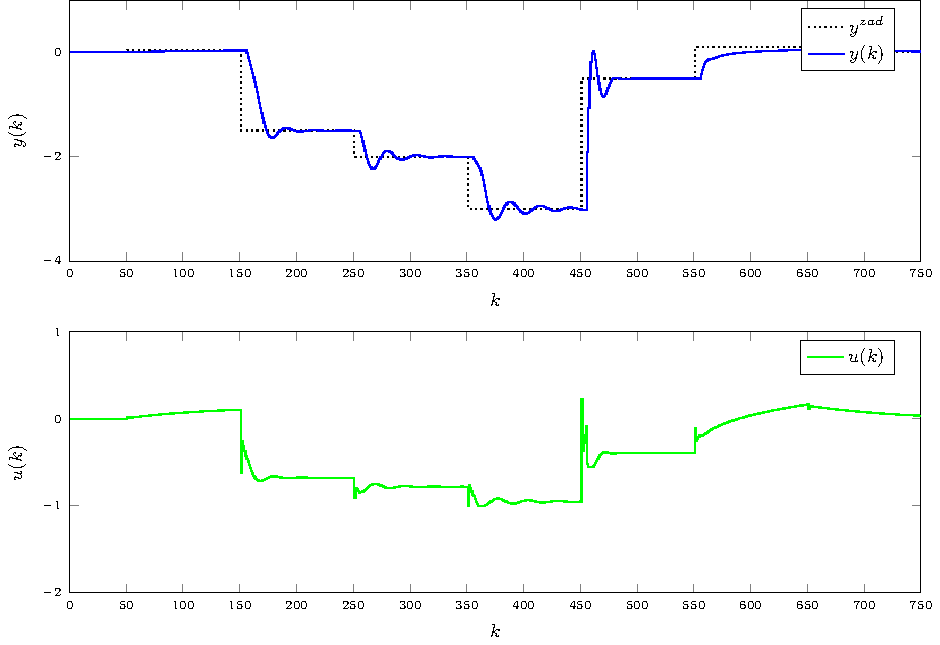
\includegraphics[width=0.2\paperwidth, height=0.15\paperheight]{data/Desired_plot_PID_number_of_fuzzy_reg_1.pdf}}
\end{figure}

Chocia� por�wnanie przebieg�w warto�ci zadanej i~warto�ci rzeczywistej nie prezentuje si� fatalnie, to wyra�nie pokazuje ono mankamenty algorytm�w liniowych.
}
			\subcolumn{0.5} \block{Kalibracja regulator�w rozmytych}{Chocia� regulatory rozmyte oferuj� znacznie wi�ksz� elastyczno�� w~kontek�cie proces�w mo�liwych do wysterowania, to jednak wprowadzj� one znaczne komplikacje w~dziedzinie doboru ich nastaw. Wynika to z~faktu, �e liczba parametr�w ro�ci w~ich przypadku liniowo wraz ze wzrostem liczby regulator�w lokalnych. Sk�adania to do postawienia tezy, �e zwi�kszanie liczby regulator�w przynosi popraw� jedynie do pewnego momentu. Ich zbyt du�a ilo��, prowadzi do b��d�w kalibracji, kt�re kompensuj� popraw� wynikaj�c� z~lepszego dopasowania regulatora do charakterystyki obiektu.

W~zwi�zku z~powy�szymi spostrze�eniami procedura doboru parametr�w musia�a by� z~g�ry zaplanowana. Regulatory testowali�my rozpoczynaj�c zawsze od jednego regulatora lokalnego. Badanie algorytmu ko�czyli�my w�wcza, gdy dalsze zwi�kszanie licbzy regulator�w skutkowa�o pogorszeniem regulacji. Ka�dy wariant kalibraowany by� w pi�ciu krokach:

\vskip 0.5cm
\begin{enumerate}
    \item R�wnomierne roz�o�enie regulator�w lokalnych w~obszarze pracy
    \item Optymalizacja parametr�w przy u�yciu algorytmu ewolucyjnego (parametry wszystkich regulator�w r�wne)
    \item Skonstruowanie dedykowanych przebieg�w warto�ci zadanej pobudzajacych obszar pracy ka�dego z~lokalnych regulator�w
    \item Indywidualna optymalizacja regulator�w ze wzgl�du na b��dy pope�niane na skonstruowanych trajektoriach
    \item R�czna poprawa parametr�w wybranych regulator�w 
\end{enumerate}
\vskip 0.5cm


}
		\end{subcolumns}

		% Central picture
		\block[]{}{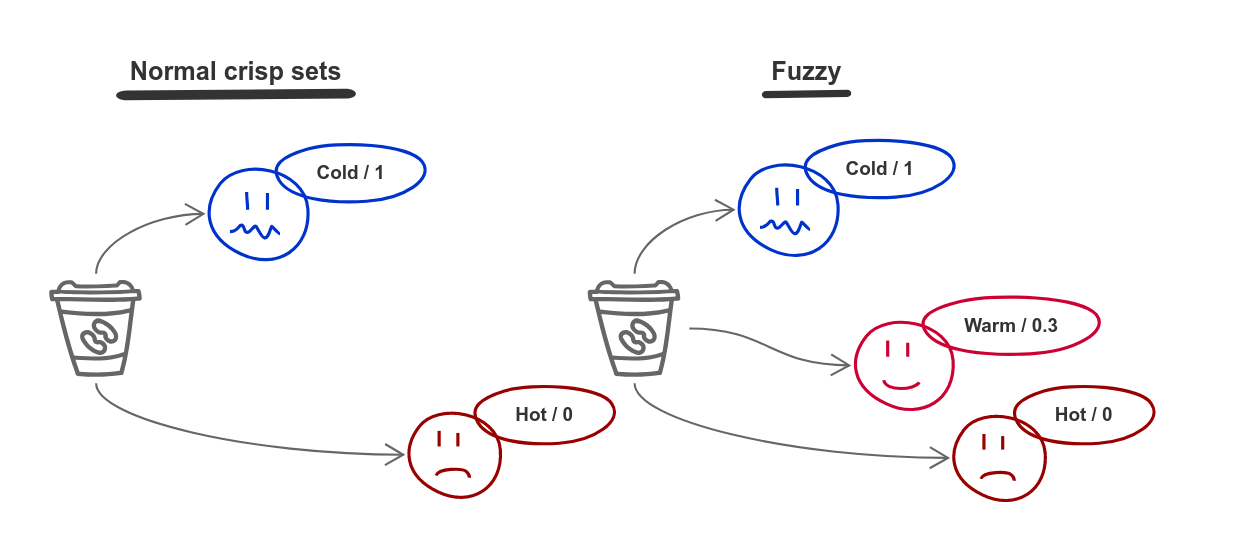
\includegraphics{img/fuzzy_poster_center_without_watermark.png}}

		% Bottom part of both 'Klasyczne regulatory PID i DMC'
		% and 'Kalibracja regulator�w rozmytych'
		\begin{subcolumns}
			\subcolumn{0.5} 
				\block[titleoffsety=0mm,bodyoffsety=-15cm]{}{Wyst�puj� wyra�ne przegulowania, czas regulacji pozostawia sporo do �yczeni, a~sygna� steruj�cy, szczeg�lnie w~ przypadku DMC, ma tendencj� do nag�ej zmiany warto�ci.

\begin{figure}[H]
    \makebox[0.21\textwidth]{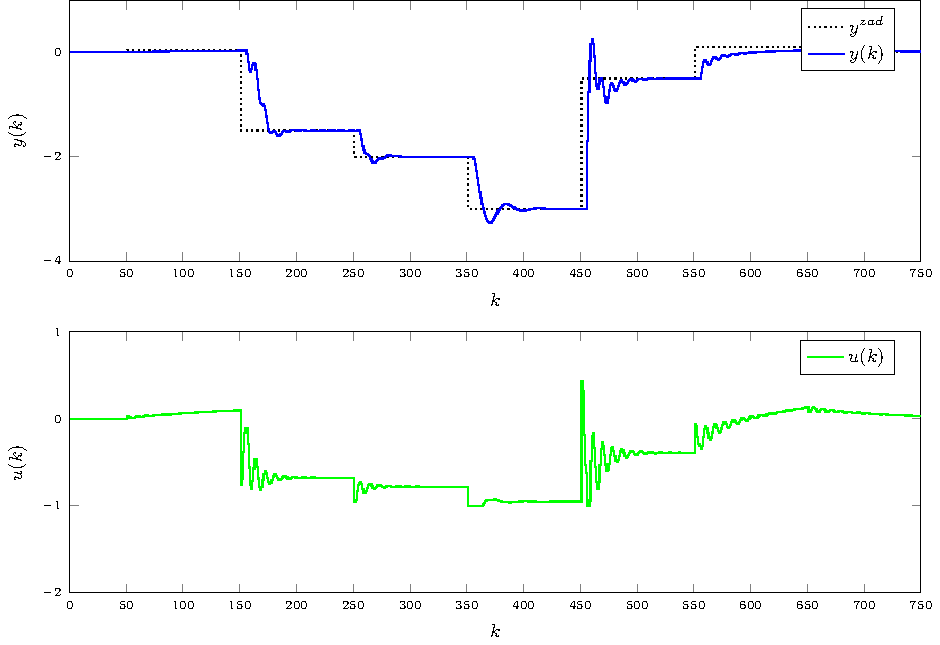
\includegraphics[width=0.2\paperwidth, height=0.15\paperheight]{data/Desired_plot_DMC_number_of_fuzzy_reg_1.pdf}}
\end{figure}

Warto zauwa�y�, �e przedstawiona trajektoria zadana jest dosy� specyficzna. Ukazuje ona tylko jedn� zmian� warto�ci zadanej o~znacznej amplitudzie, co nie pozwala dostrzec zachowania regulator�w przy jej znacznej w~przeciwnym kierunku. Najprawdopodobniej przy szerszym spektrum zmian regulatory ukaza�yby swoj� niedoskona�o�� w~znacznie wi�kszym stopniu.

}	
			\subcolumn{0.5} 
				\block[bodyoffsety=-15cm]{}{Sprecyzowany schemat post�powania powoli� nam obiektywnie por�wnywa� poszczeg�lne warianty i~znacznie przyspieszy� prowadzenie bada�. Na tym etapie warto podkre�li�, �e jako \textit{zmienna rozmywaj�ca} wybrana zosta� warto�� wyj�ciowa obiektu. Przeprowadzone eksprytmenty pokaza�y, �e prowadzi to do poprawienia jako�ci regulacji, co da�o si� przewidzie� ju� na etapie analizy charakterystyki statycznej obiektu. Dalsze badania potwierdzi�y stawian� tez�, co przedstawia poni�szy wykres. Pewien niepok�j mo�e powodowa� fakt zwi�kszenia b��du przy 4 regulatorach DMC, jednak by�o to spowodowane nieoptymalnym rozlokowaniem regulator�w na danym zakresie sterowania (regulatory rozlokowane by�y w r�wnych odst�pach).

\vskip 1cm
\begin{figure}[H]
        \begin{tikzpicture}
            \begin{axis}[
                    width=0.20\textwidth,
                    height=0.1\textheight,
                    xmin=0,xmax=6,ymin=60,ymax=100,
                    xlabel={liczba regulator�w},
                    ylabel={error},
                    xtick={0,1,2,3,4,5,6},
                    legend pos=south east,
                    legend style={font=\tiny},
                    y tick label style={/pgf/number format/1000 sep={,}},
                ]
                
                \addplot[mark=o,draw=blue]               file {data/DMC_error.txt};
                \addplot[mark=o,draw=red]               file {data/PID_error.txt};

                \legend{DMC error, PID error}
            \end{axis}
        \end{tikzpicture}
        \label{DMC_PIS_error}
\end{figure}
\vskip 1cm}
		\end{subcolumns}

	% Third COLUMN
	\column{0.25}

		\block{Wyniki regulacji rozmytej}{Zgodnie z~przewidywaniami, rozmycie regulator�w liniowych pozwoli�o uzyska� zauwa�alnie, chocia� nie nadzwyczajnie lepsz� jako�� regulacji. Podstaw� oceny jako�ci regulacji by� sumaryczny b��d kwadratowy pope�niany przez regulator w~trakcie symulacji. W~mniejszym stopniu brany by� tak�e pod uwag� charakter przebiegu warto�ci steruj�cej.

Rozmywanie regulatora PID zako�czyli�my na \textbf{5 regulatorach rozmytych}. W~tej konfiguracji uzyskali�my najmniejszy b��d regulacji. Przy wszystkich zmianach warto�ci zadanej wyra�nie zmniejszone zosta�o przeregulowanie, co jest nierzadko jednym z~najwa�niejszych kryteri�w regulacji. Ponadto, w~dolnych partiach charakterystyki uda�o si� uzyska� znaczne skr�cenie czasu regulacji. Jedynie przy widocznym na wykresie skoku warto�ci zadanej w~kierunku dodatnim, czas regulacji wyd�u�y� si�.

\vskip 1cm
    \begin{figure}[H]
        \makebox[0.21\textwidth]{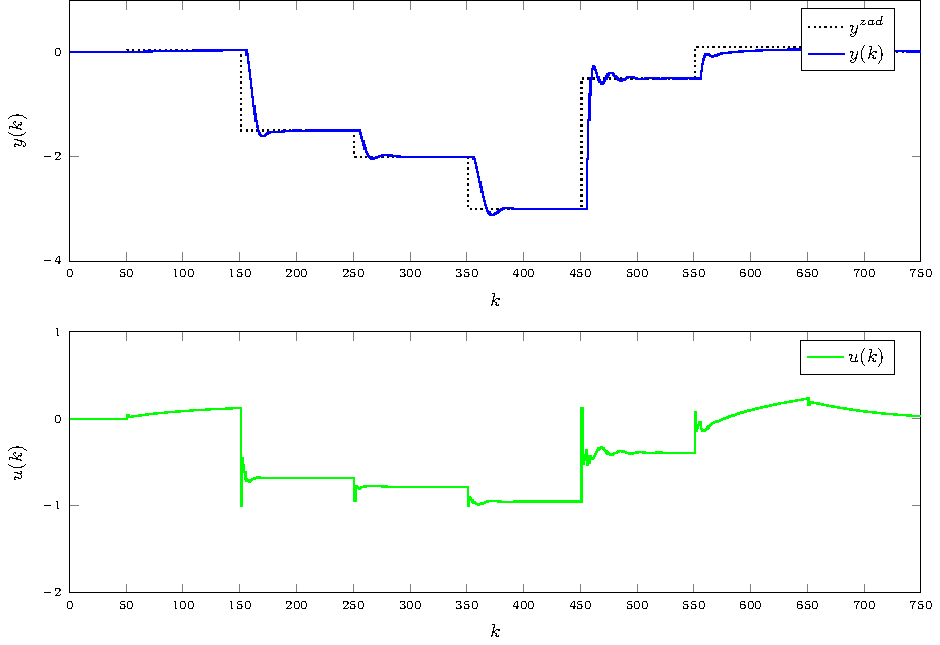
\includegraphics[width=0.2\paperwidth, height=0.15\paperheight]{data/Desired_plot_PID_number_of_fuzzy_reg_5.pdf}}
    \end{figure}
    \vskip 1cm

Wi�ksz� popraw� zauwa�y� mo�na przy por�wnaniu klasycznej i~rozmytej wersji regulatora DMC. Dzi�ki \textbf{zwi�kszeniu liczby regulator�w lokalnych do 3} uzyskali�my znaczne zmniejszenie przeregulowania oraz skr�cenie czasu regulacji przy ka�dym ze skok�w warto�ci zadanej. R�wnie� przebieg sygna�u steruj�cego charakteryzuje si� zmniejszonymi oscylacjami oraz szybszym czasem stabilizacji. 


\vskip 1cm
    \begin{figure}[H]
        \makebox[0.21\textwidth]{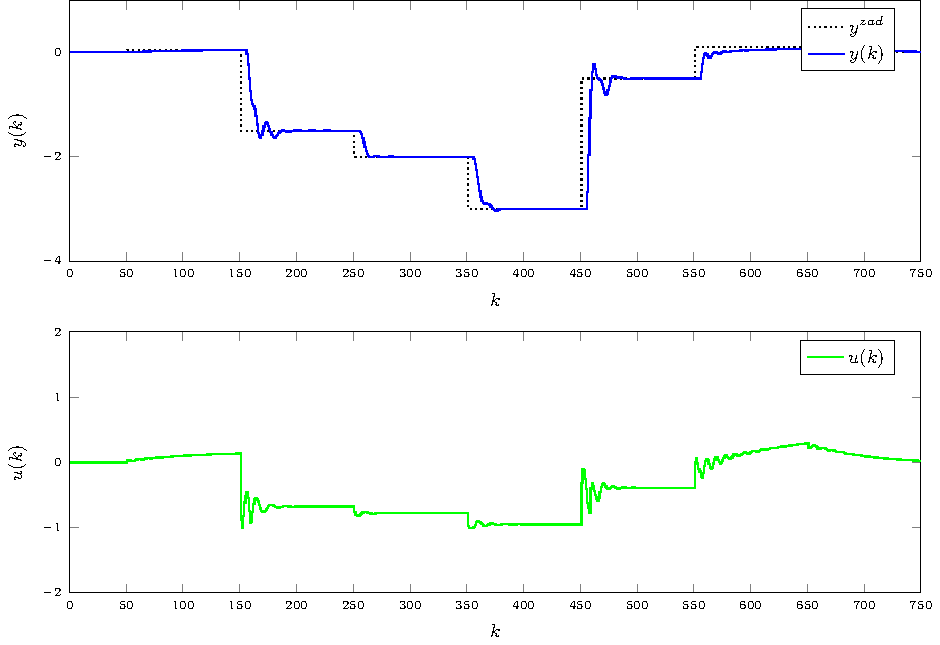
\includegraphics[width=0.2\paperwidth, height=0.15\paperheight]{data/Desired_plot_DMC_number_of_fuzzy_reg_3.pdf}}
    \end{figure}
\vskip 1cm

Uzyskane przez nas wyniki jednoznacznie pokazuj� zastosowanie teorii zbior�w rozmytych w~zadaniu regulacji obiekt�w nieliniowych przyczyni� si� mo�e do poprawy jako�ci sterowania. Jednocze�nie zabieg ten nie jest okupiony du�ym wzrostem skomplikowania idei sterowania, poniewa� in�ynier wci�� ma do czynienia ze standardowymi regulatorami liniowymi tylko, �e w~wi�kszej liczbie.}
		\block{Podsumowanie}{Logika rozmyta zosta�a wprowadzona do powszechnego obiegu w~latach 60' ubieg�ego wieku, chocia� wcze�niej zajmowali si� ni� takie osobisto�ci jak prof. Jan �ukasiewicz czy prof. Alfred Tarski. Od tamtej pory znalaz�a ona zastosowania w~szeregu r�nych dziedzin poczynaj�c od analizy mowy, przez podejmowanie decyzji medycznych czy biznesowych, na autonomicznych systemach obronnych ko�cz�c. Swoje miejsce zaj�a tak�e w~dziedzinie szeroko poj�tego sterowania.

Wykorzystanie logiki rozmytej pozwala nie tylko modelowa� procesy nieliniowe z~pomoc� kilku dobrze znanych, liniowych modeli, ale umo�liwia tak�e matematyczne uj�cie nieprecyzyjnej ("rozmytej") wiedzy eksperckiej. Po��czona z~innymi, dobrze przeanalizowanymi na przestrzeni dekad, metodami regulacji stanowi ona pot�ne narz�dzie w~r�kach wsp�czesnych in�ynier�w. Jej przyk�ad pokazuje, �e na r�wni z~post�puj�cym rozwojem technologii, wa�ne jest rozwijanie solidnych podstaw matematycznych, poniewa� to one zapewniaj� nam wydajne wykorzystanie posiadanych zaspob�w obliczeniowych.}

\end{columns}

% Footer
\node [above right,font=\small] at (bottomleft) {Autorzy: Pawe� Bugyi, Marcin Michalski, Krzysztof Pierczyk. Wykorzystana grafika ze strony: https://towardsdatascience.com/fuzzy-logic-and-how-it-is-curing-cancer-dc6bcc961ded};

\end{document}
\endinput
